\section{Implementation}

\begin{frame}
	\frametitle{The Barnes-Hut Approximation}
	\begin{enumerate}
		\item Place all the particles in a tree.
		\item For each tree node, compute the center of mass.
		\item For each particle, compute a force. Start interacting with the root level, request deeper levels if
		$$\theta<\frac{s}{d}.$$
		\item Perform a time step.
		\item \emph{Update} the tree structure.
		\item Save results if needed, go to 2 or exit.
	\end{enumerate}
\end{frame}

\begin{frame}
	\frametitle{The Barnes-Hut (Quad-)Tree}
	\begin{figure}
		\centering
		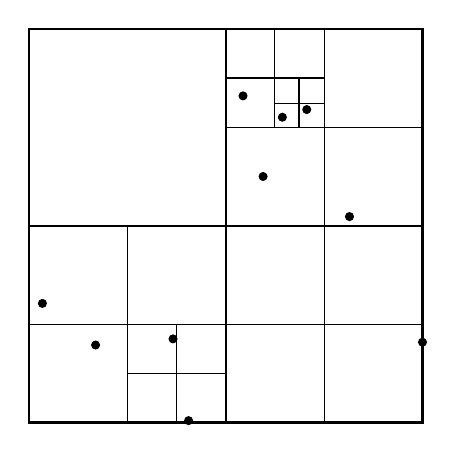
\begin{tikzpicture}[scale=0.05,%
		every circle node/.style = {width=3,fill=black}]
		
% Simulation domain
\draw[thick] (0,0) rectangle (100,100);
\pause
% Level 1
\draw[thick] (50,0) -- (50,100);
\draw[thick] (0,50) -- (100,50);
\draw[fill] (16.9664,19.6802) circle (1); %0
\pause
\draw[fill] (54.4110,82.9573) circle (1); %1
\pause
\draw (0,25) -- (50,25);
\draw (25,0) -- (25,50);
\draw[fill] (03.4614,30.2489) circle (1); %2
\pause
% Level 2
\draw (0,25) -- (100,25);
\draw (75,0) -- (75,100);
\draw (25,0) -- (25,50);
\draw (50,75)-- (100,75);
% Level 3
\draw (25,12.5) -- (50,12.5);
\draw (37.5,0)  -- (37.5,25);
\draw (62.5,75) -- (62.5,100);
\draw (50,87.5) -- (75,87.5);
% Level 4
\draw[thin] (68.625,75) -- (68.625,87.5);
\draw[thin] (62.5,81.125) -- (75,81.125);
% Particles (by increasing id)
\draw[fill] (81.4564,52.3018) circle (1); %3
\draw[fill](59.5102,62.4865) circle (1);  %4
\draw[fill] (40.5800,00.4751) circle (1); %5
\draw[fill] (64.4035,77.5371) circle (1); %6
\draw[fill] (36.6343,21.2396) circle (1); %7
\draw[fill] (99.9970,20.3979) circle (1); %8
\draw[fill] (70.6045,79.4802) circle (1); %9
		\end{tikzpicture}
		\caption{Sample 4-level Barnes-Hut grid with 10 particles.}
		\label{fig:bh-grid}
	\end{figure}
\end{frame}

\begin{frame}
	\frametitle{The Barnes-Hut (Quad-)Tree (Cont.)}
	\begin{figure}
		\centering
		\newlength{\lvld}
		\setlength{\lvld}{7em}
		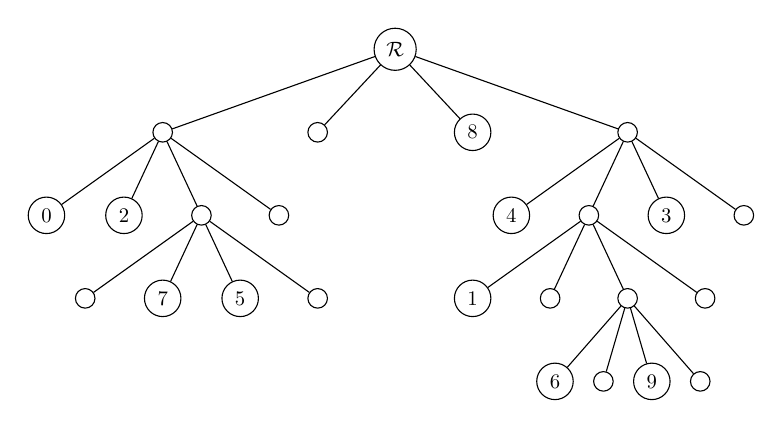
\begin{tikzpicture}[level distance=3em,
		sibling distance=3em,
		level 1/.style={sibling distance=0.80\lvld},
		level 2/.style={sibling distance=0.40\lvld},
		level 3/.style={sibling distance=0.4\lvld},
		level 4/.style={sibling distance=0.25\lvld},
		every node/.style = {shape=circle, draw, align=center, color=black,
			fill=white, scale=0.75}]
		\node {$\mathcal{R}$} %Root
child { node {} %1SW
	child { node{0} } %2SW
	child { node{2} } %2NW
	child { node{} %2SE
		child { node{} } %3SW
		child { node{7} } %3NW
		child { node{5} } %3SE
		child { node{} } } %3NE
	child { node{} } } %2NE
child { node{} }%1NW
child { node{8} }%1SE
child { node{} %1NE
	child { node{4} } %2SW
	child { node{} %2NW
		child { node {1} } %3SW
		child { node {} } %3NW
		child { node {} %3SE
			child { node{6} } %4SW
			child { node{} } %4NW
			child { node{9} } %4SE
			child { node{} } %4SW
		}
		child { node {} } }%3NE
	child { node{3} } %2SE
	child{ node{} } }; %2NE
		\end{tikzpicture}
		\caption{Tree structure associated to the configuration depicted in \cref{fig:bh-grid}.}
	\end{figure}
\end{frame}

\begin{frame}
	\frametitle{Data Structures}
	To compute forces, all we need is information about the centers of mass. In the code,
	\begin{itemize}
		\item A \lstinline{Particle} describes a center of mass (mass, position, velocity, acceleration).
		\item A \lstinline{Node} is a \lstinline{Particle} wrapper. It gives a center of mass information about its surrounding (geometrical boundaries, parent, children).
		\item A \lstinline{QuadTree} manages \lstinline{Node} objects. It provides methods to browse the tree.
		\item A \lstinline{Simulation} manages the run, times it (with \lstinline|Timer|) including IO (via \lstinline{IOManager}).
	\end{itemize}
\end{frame}

\begin{frame}
	\frametitle{Data Structures (Cont.)}
	\begin{figure}
		\centering
		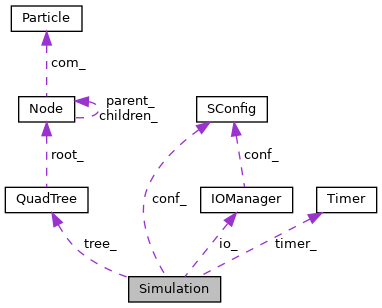
\includegraphics[width=0.5\textwidth]{inclfigs/class_simulation.png}
		\caption{Collaboration graph of the \lstinline|Simulation| class.}
	\end{figure}
\end{frame}

\begin{frame}
	\frametitle{Data Structures (Cont.)}
	Computation of the force should be the main task. Avoid memory latency issues if possible?
	\begin{itemize}
		\item<1-> SoA vs. \only<1>{AoS}\only<2->{\alert{AoS}}: SoA feasible on one CPU. However,
		\begin{itemize}
			\item Parallelized problem managing only some particles?
			\item Particles being passed after time evolution?
			\item Runaway particles?
		\end{itemize}
		\item<2-> \only<2>{Pointers}\only<3->{\alert{Pointers}} or array in the tree?
		\begin{itemize}
			\item Inhomogeneous particle distributions, most nodes empty.
			\item Using arrays means allocating full levels, exponentially increasing memory usage.
		\end{itemize}
	\end{itemize}

	\onslide<3->{However, the ``physical'' particles being simulated are kept local to another in a separate storage (in \lstinline|SConfig|).}
\end{frame}

\begin{frame}
\frametitle{Recursion}
Up to v0.5 (FMM attempt), code was written with recursive instructions. For example:

\end{frame}
